\documentclass[12pt]{article}
\usepackage[T1]{fontenc}
\usepackage[T1]{polski}
\usepackage[utf8]{inputenc}
\usepackage{graphicx}
\usepackage{amsfonts}
\usepackage{float}

\setlength{\textheight}{20cm}

\title{{\bf Zadanie nr 4 -Przekształcenie Fouriera, Walsha-Hadamarda, kosinusowe i falkowe,
szybkie algorytmy.}\linebreak
Cyfrowe Przetwarzanie Sygnałów}
\author{Krzysztof Barden, 210139 \and Paweł Galewicz, 210182}
\date{14.06.2019r.}

\begin{document}
\clearpage\maketitle
\thispagestyle{empty}
\newpage
\setcounter{page}{1}
\section{Cel zadania}

Celem ćwiczenia jest zapoznanie się z operacjami transformacji sygnałów dyskretnych
przy użyciu wybranych metod.
Pierwszy wykres jest wykresem sygnału transformowanego.
Możliwe są dwa tryby prezentacji wykresów. 
\begin{itemize}
\item (W1) – górny wykres prezentuje część rzeczywistą amplitudy w funkcji
częstotliwości, a wykres dolny część urojoną;
\item (W2) – górny wykres prezentuje moduł liczby zespolonej, a dolny argument liczby
w funkcji częstotliwości.
 splotu.
\end{itemize}

\section{Wstęp teoretyczny}

Program z zadania 1 ,2  i 3 został rozszerzony o dodadtkowe funkcjonalnosci. Wykresy generowane są przy użyciu biblioteki LiveCharts \cite{lv}. GUI aplikacji zostało stworzone przy użyciu biblioteki WPF \cite{wpf}.
\\Interfejs został rozszerzony o interfejs transjormacji sygnałów oraz o interfejs filtrów:
\begin{figure}[H]
 \centering
 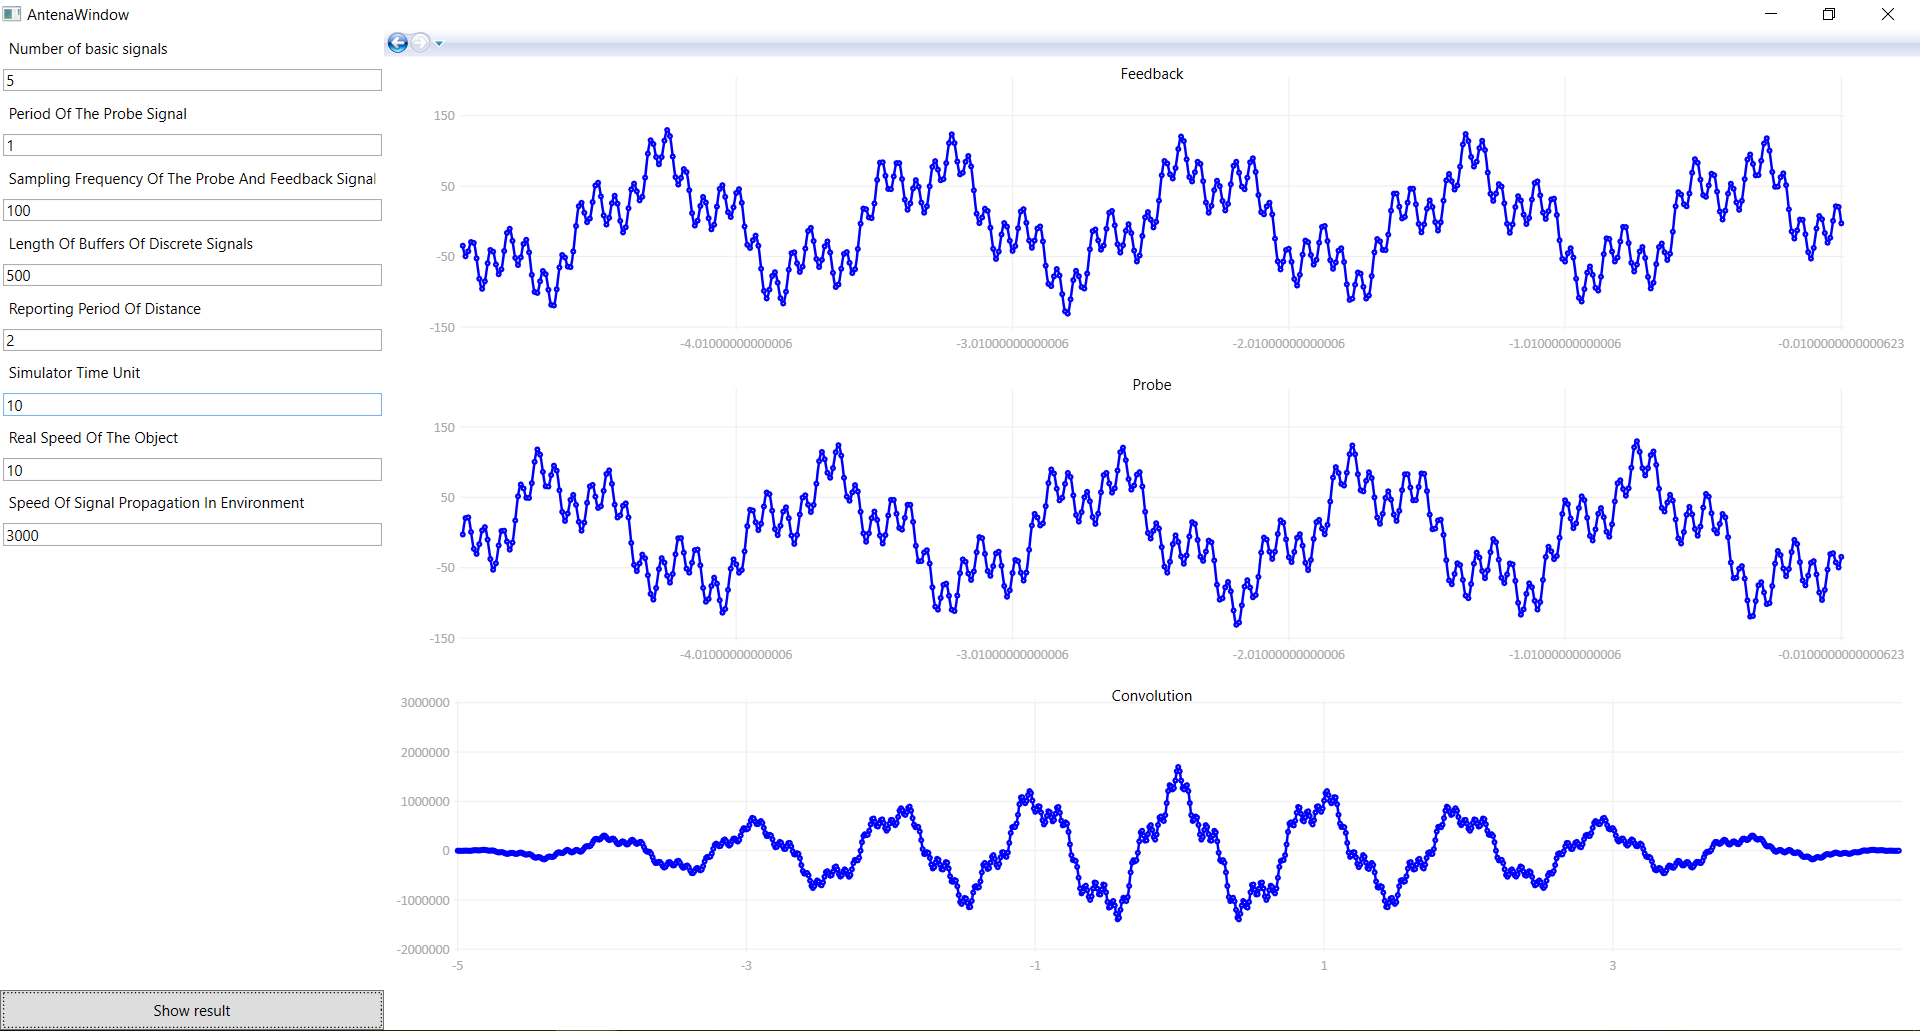
\includegraphics[width=15cm]{images/antenaWindow.PNG}
 \vspace{-0.3cm}
 \caption{Interfejs graficzny anteny}
 \label{gui}
\end{figure}
\begin{figure}[H]
 \centering
 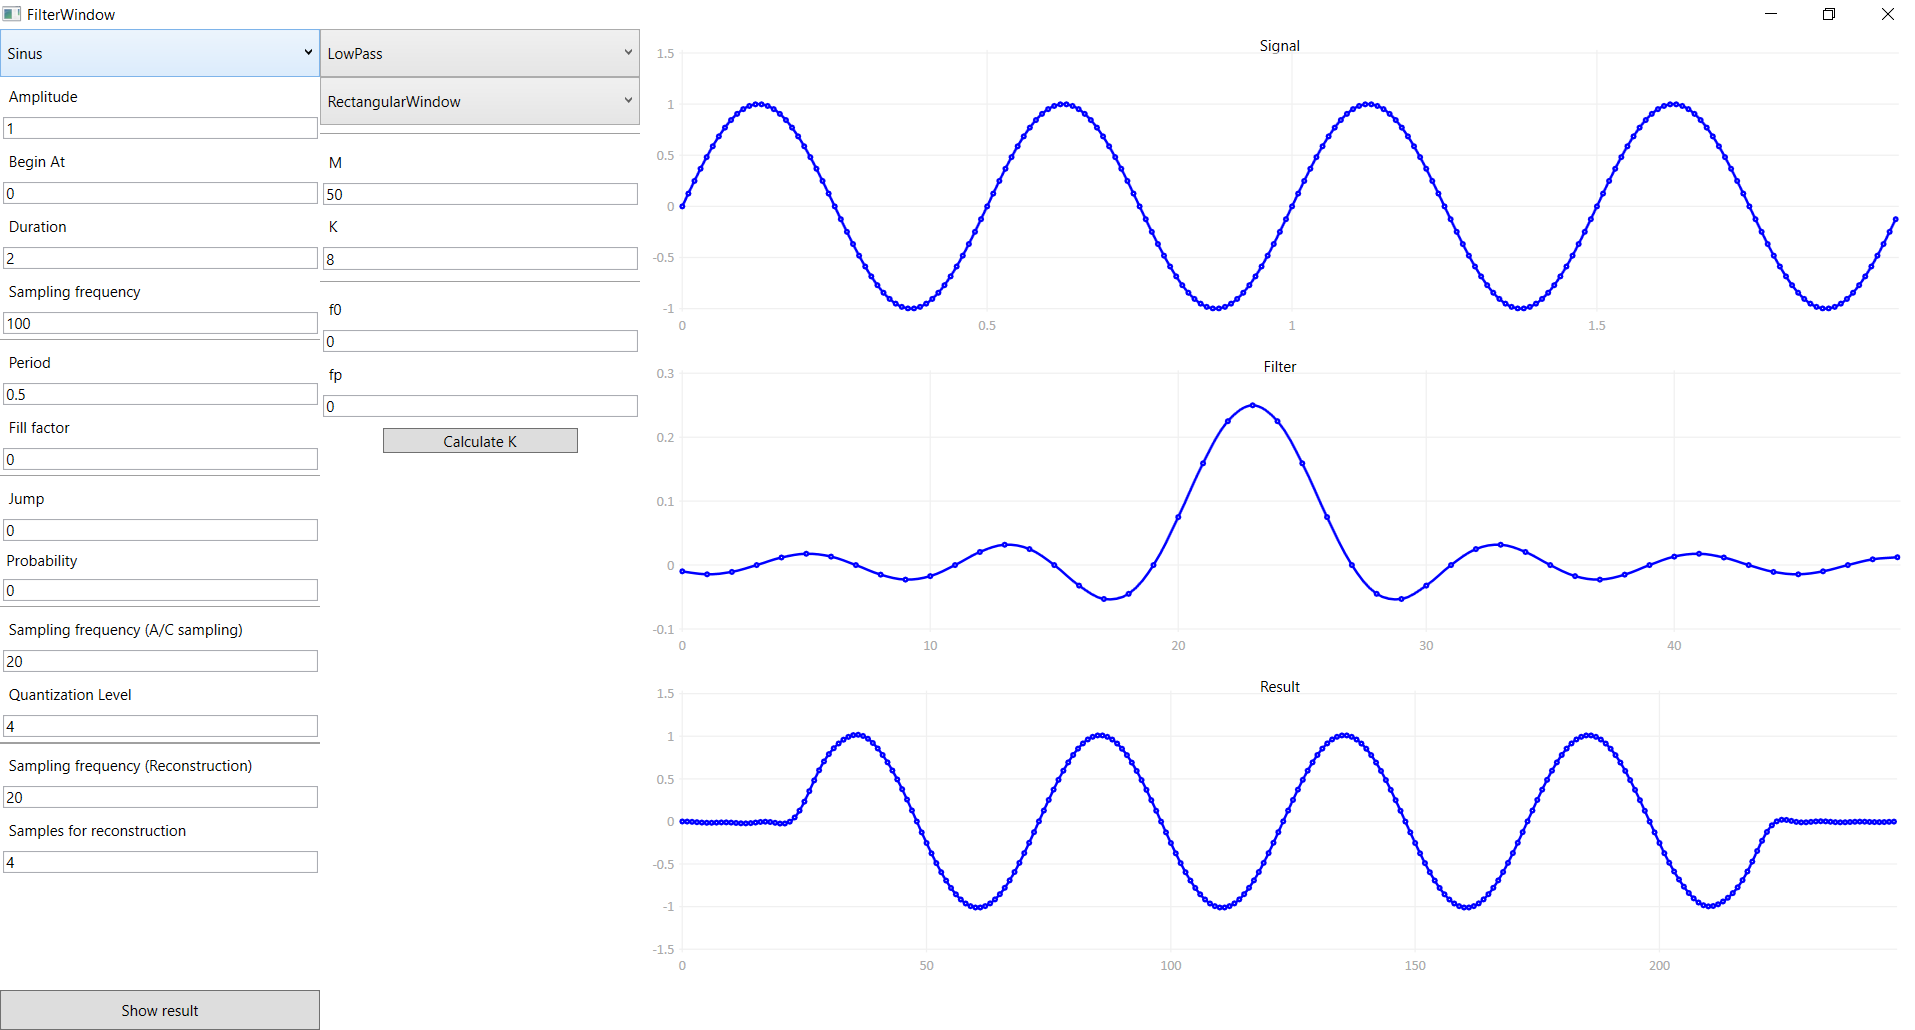
\includegraphics[width=15cm]{images/filterWindow.PNG}
 \vspace{-0.3cm}
 \caption{Interfejs graficzny filtracji}
 \label{gui}
\end{figure}


Aby wygenerować sygnały należy w lewej kolumnie wypełnić parametry i nacisnąć przycisk "i". 
\section{Eksperymenty i wyniki}


%%%%%%%%%%%%%%%%%%%%%%%%%%%%%%%%%%%%%%%%%%%%%%%%%%%%%%%%%%%%%%%%%%%%%%%%%%%%%%%%%%%%%%%%%%%%%%%%%%%%%%%%%%%%%%%%%
% PODROZDZIAŁ PT. EKSPERYMENT NR 1 
%%%%%%%%%%%%%%%%%%%%%%%%%%%%%%%%%%%%%%%%%%%%%%%%%%%%%%%%%%%%%%%%%%%%%%%%%%%%%%%%%%%%%%%%%%%%%%%%%%%%%%%%%%%%%%%%%

\subsection{Eksperyment nr 1 }
\subsubsection{Filtracja sygnałów}
Celem tego eksperymentu zaprezentowanie możliwosci programu do wykonania filtracji sygnałów

\subsubsection{Rezultat}
\begin{figure}[H]
 \centering
 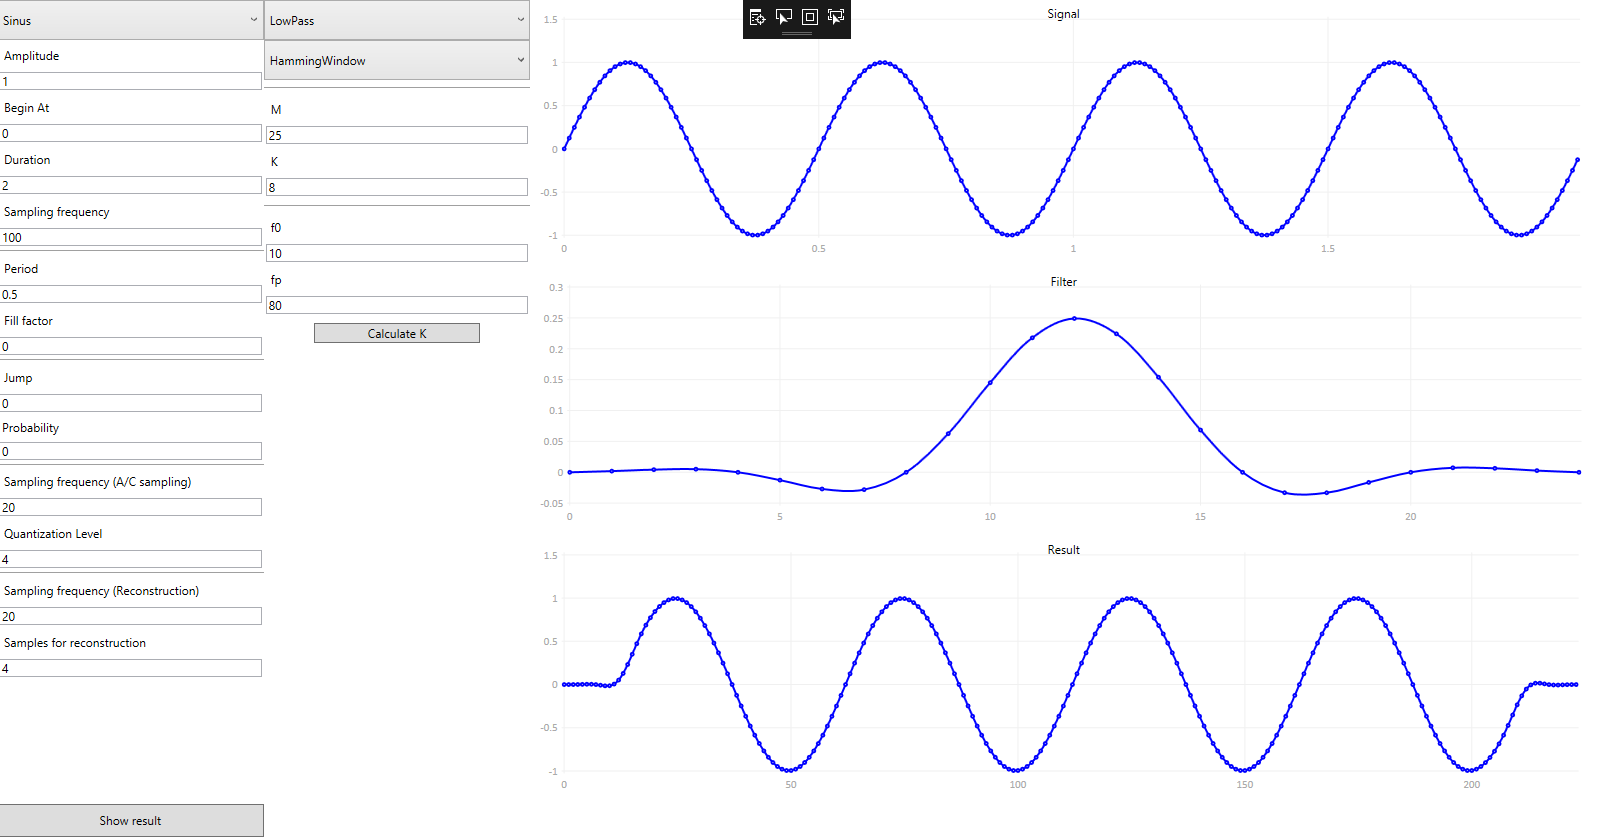
\includegraphics[width=14cm]{images/lowham.PNG}
 \vspace{-0.3cm}
 \caption{Filtracja dolnoprzepustowa z oknem Hamminga}
 \label{gui}
\end{figure}
\begin{figure}[H]
 \centering
 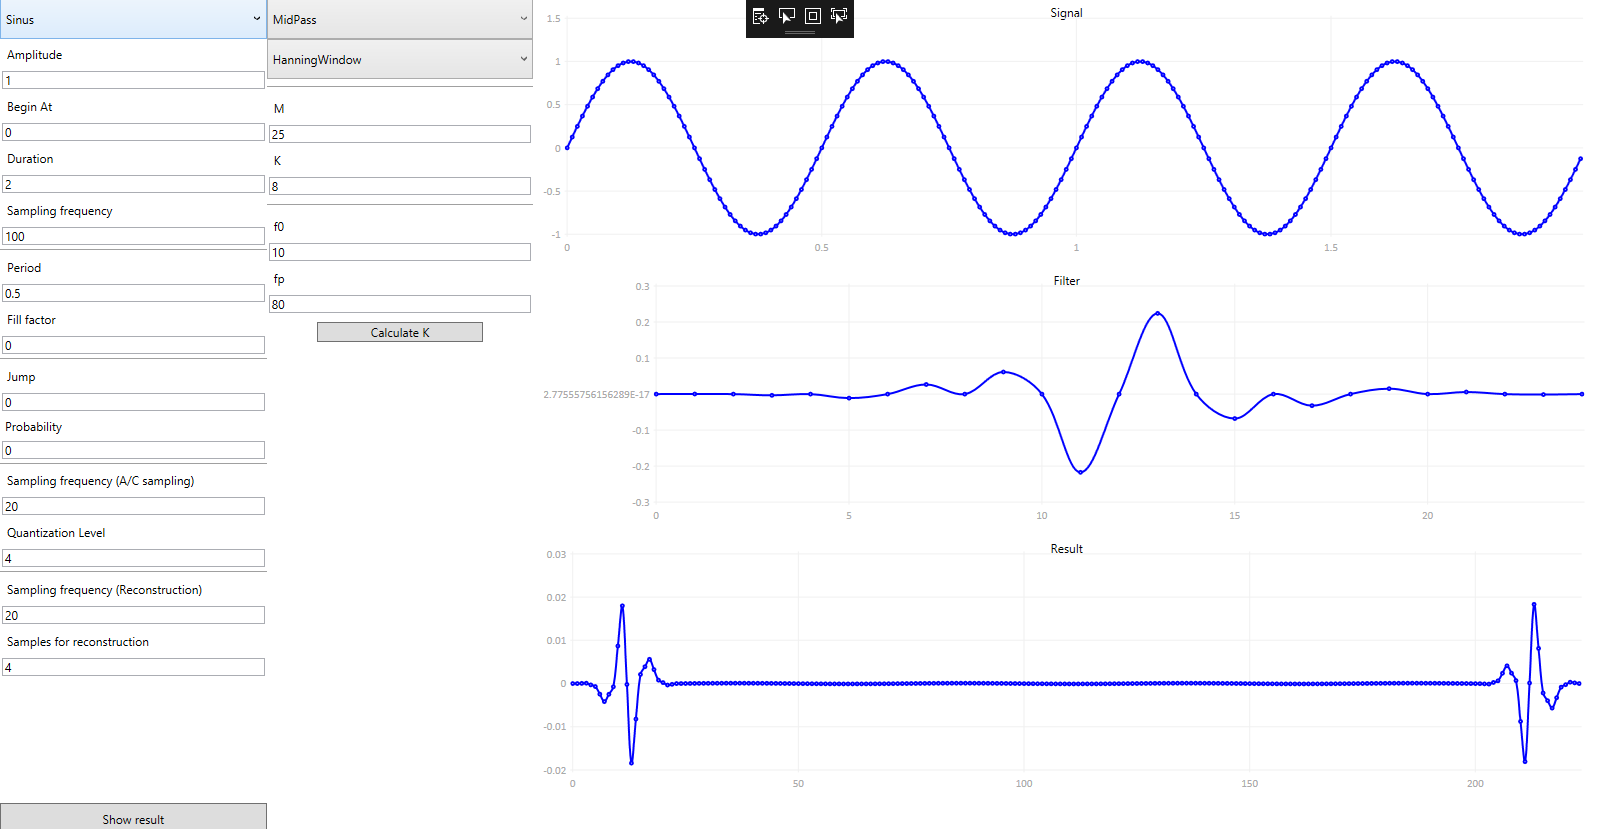
\includegraphics[width=14cm]{images/midhan.PNG}
 \vspace{-0.3cm}
 \caption{Filtracja srodkowoprzepustowa z oknem prostokątnym}
 \label{gui}
\end{figure}
\begin{figure}[H]
 \centering
 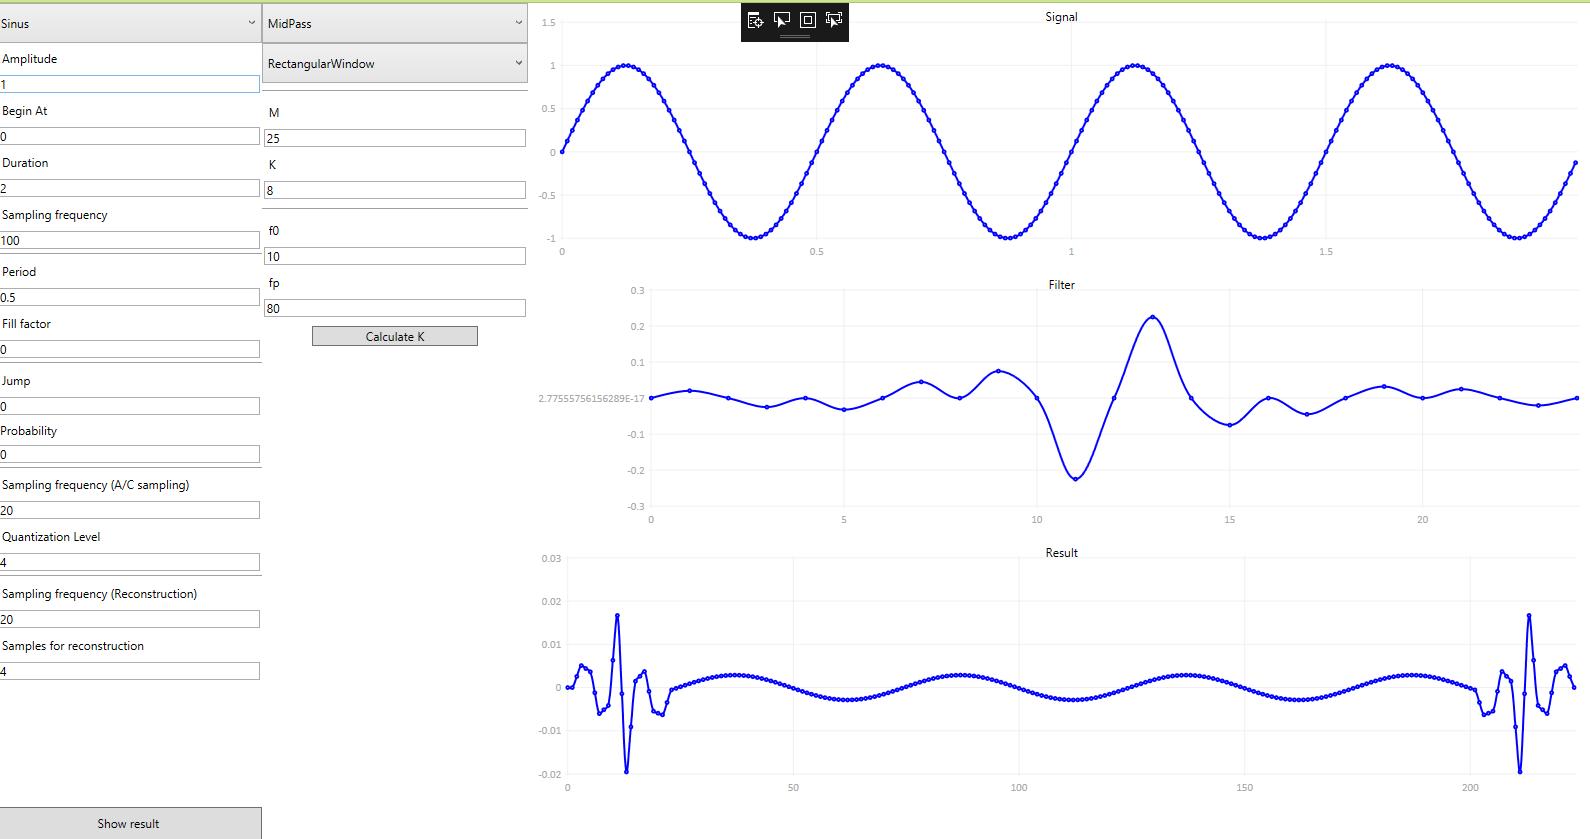
\includegraphics[width=14cm]{images/midrect.PNG}
 \vspace{-0.3cm}
 \caption{Filtracja srodkowoprzepustowa z oknem Hanninga}
 \label{gui}
\end{figure}
\begin{figure}[H]
 \centering
 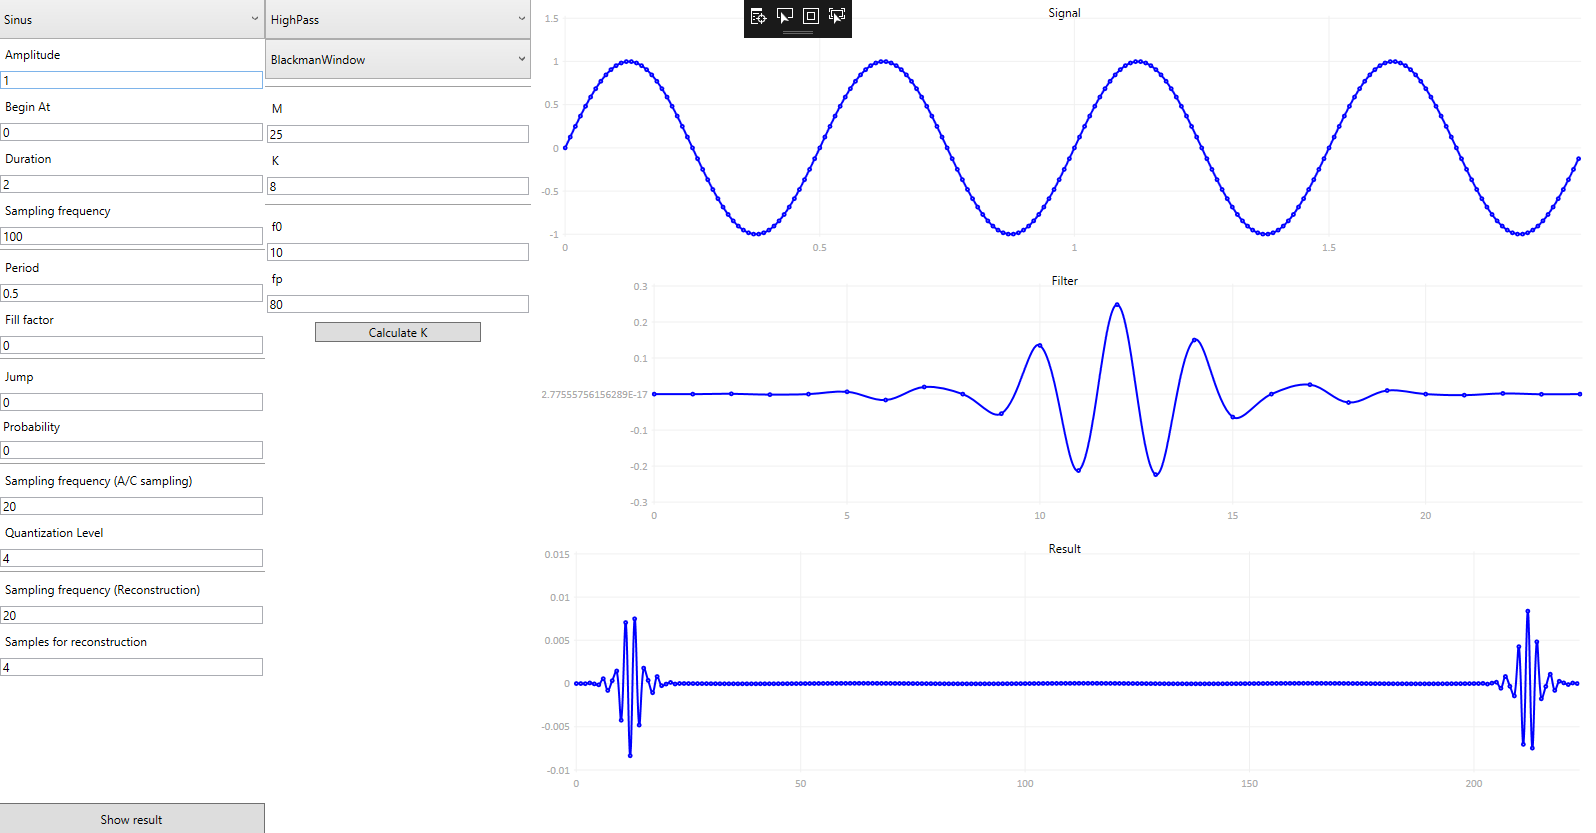
\includegraphics[width=14cm]{images/highblack.PNG}
 \vspace{-0.3cm}
 \caption{Filtracja górnoprzepustowa z oknem Blackmana}
 \label{gui}
\end{figure}

%%%%%%%%%%%%%%%%%%%%%%%%%%%%%%%%%%%%%%%%%%%%%%%%%%%%%%%%%%%%%%%%%%%%%%%%%%%%%%%%%%%%%%%%%%%%%%%%%%%%%%%%%%%%%%%%%
% PODROZDZIAŁ PT. EKSPERYMENT NR 2
%%%%%%%%%%%%%%%%%%%%%%%%%%%%%%%%%%%%%%%%%%%%%%%%%%%%%%%%%%%%%%%%%%%%%%%%%%%%%%%%%%%%%%%%%%%%%%%%%%%%%%%%%%%%%%%%%

\subsection{Eksperyment nr 2 }
\subsubsection{Operacja splotu i korelacji}
Celem tego eksperymentu było zaprezenotwanie możliwosći programu do wykonania operacji splotu i korelacji

\subsubsection{Rezultat}

\begin{figure}[H]
 \centering
 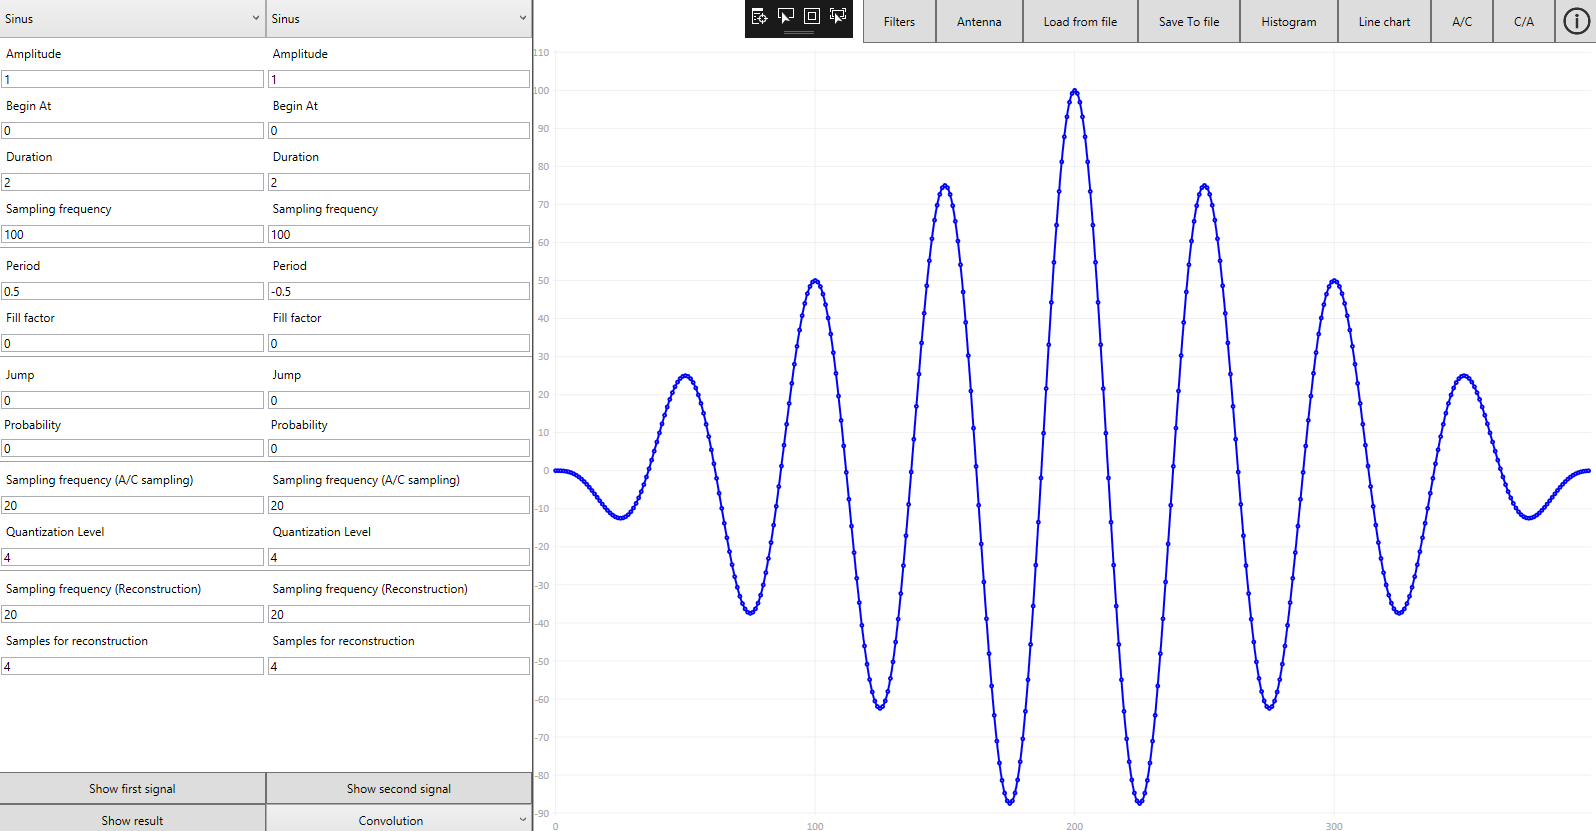
\includegraphics[width=14cm]{images/conv.PNG}
 \vspace{-0.3cm}
 \caption{Wykres wyniku operacji splotu}
 \label{gui}
\end{figure}
\begin{figure}[H]
 \centering
 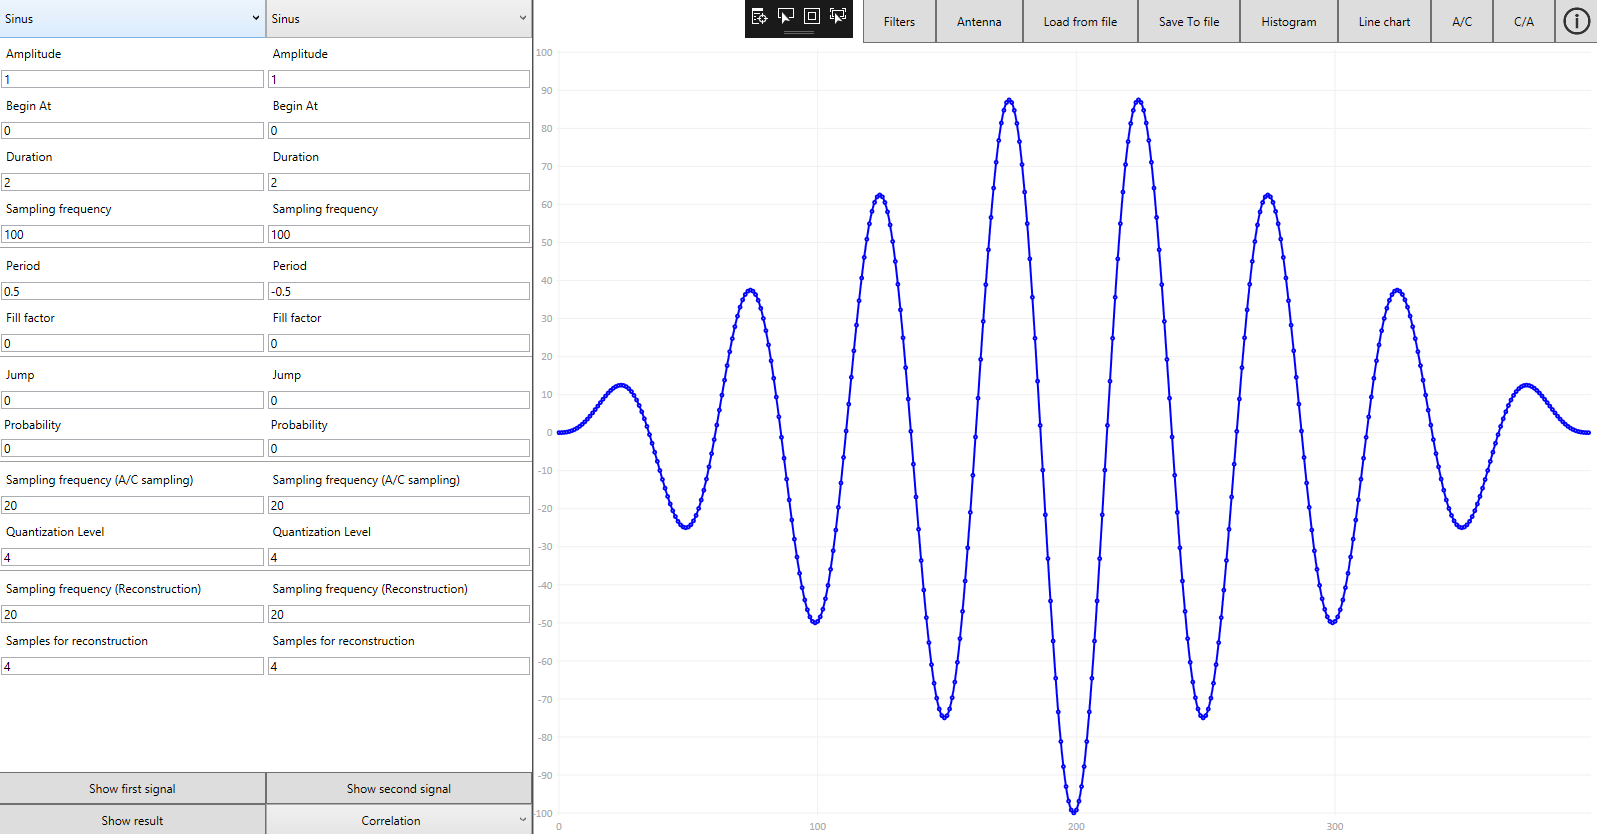
\includegraphics[width=14cm]{images/corel.PNG}
 \vspace{-0.3cm}
 \caption{Wykres wyniku operacji korelacji}
 \label{gui}
\end{figure}
\begin{figure}[H]
 \centering
 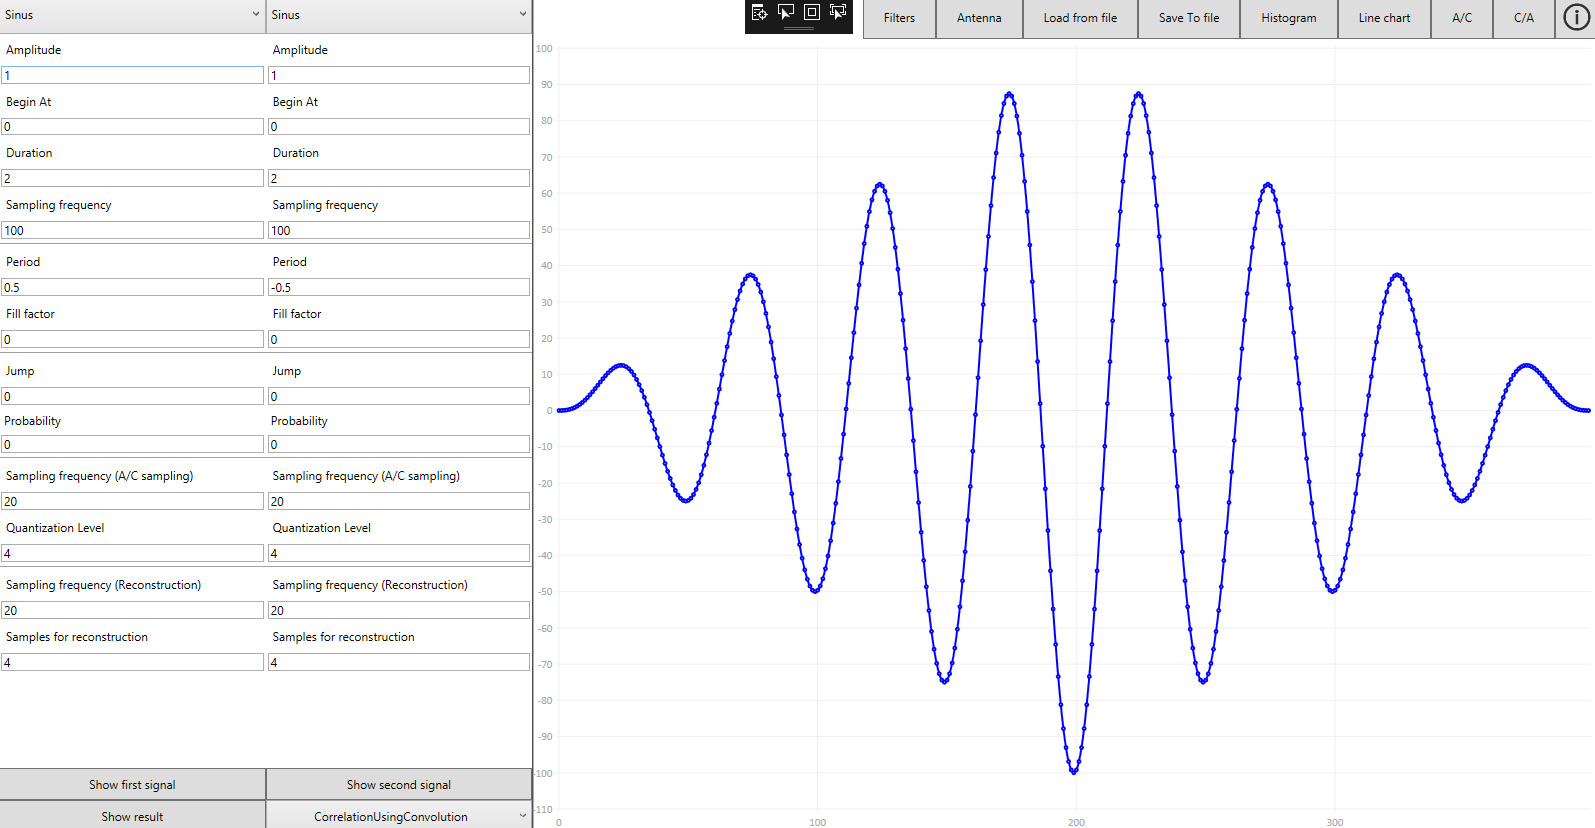
\includegraphics[width=14cm]{images/corelconv.PNG}
 \vspace{-0.3cm}
 \caption{Wykres wyniku operacji korelacji wyliczonej za pomocą operacji splotu}
 \label{gui}
\end{figure}





%%%%%%%%%%%%%%%%%%%%%%%%%%%%%%%%%%%%%%%%%%%%%%%%%%%%%%%%%%%%%%%%%%%%%%%%%%%%%%%%%%%%%%%%%%%%%%%%%%%%%%%%%%%%%%%%%
% PODROZDZIAŁ PT. EKSPERYMENT NR 3
%%%%%%%%%%%%%%%%%%%%%%%%%%%%%%%%%%%%%%%%%%%%%%%%%%%%%%%%%%%%%%%%%%%%%%%%%%%%%%%%%%%%%%%%%%%%%%%%%%%%%%%%%%%%%%%%%




\subsection{Eksperyment nr 3 }
\subsubsection{Korelacyjny czujnik odległosci}
Do zaprezentowania możliwosci korelacyjnego czujnika odległosci przedstawimy eksperyment w którym dokonamy pomiarów dla 3 sygnałów, każdy z innymi parametrami sygnałów.


\subsubsection{Rezultat}

\begin{figure}[H]
 \centering
 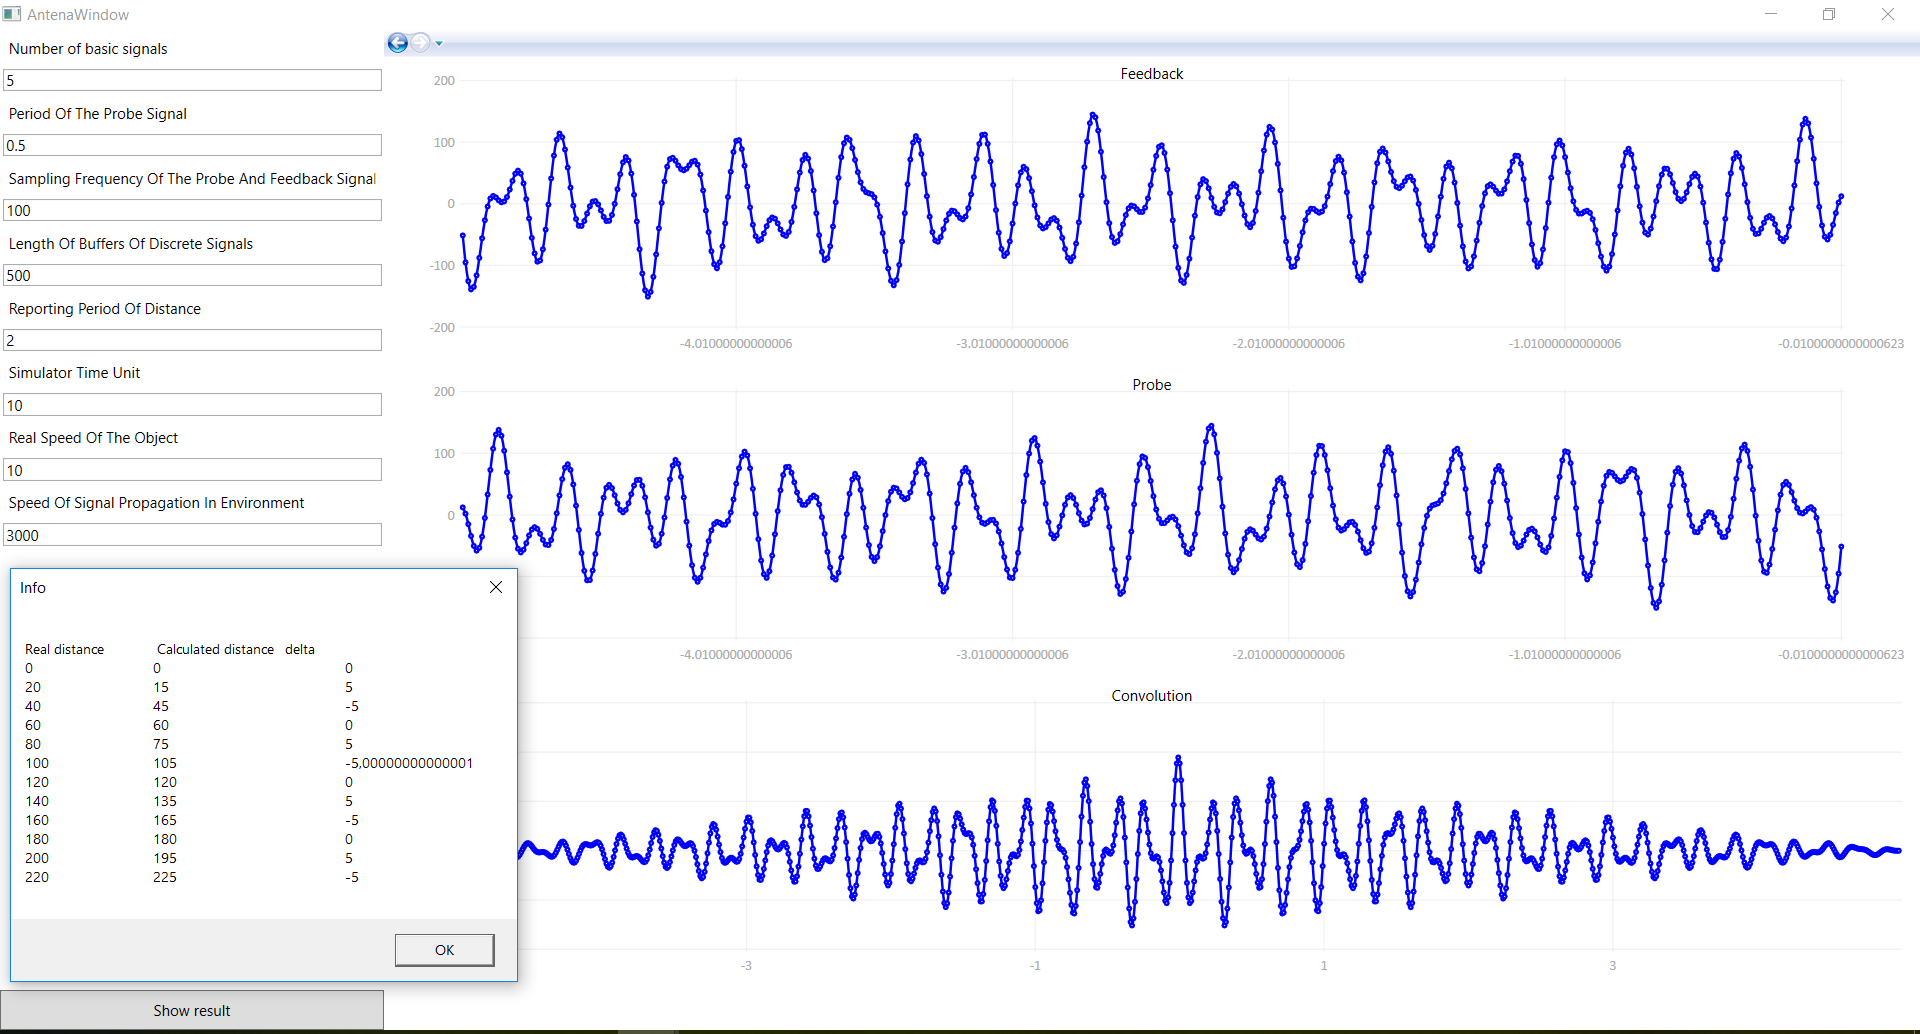
\includegraphics[width=14cm]{images/a1.PNG}
 \vspace{-0.3cm}
 \caption{Korelacyjny czujnik odległosci}
 \label{gui}
\end{figure}

\begin{figure}[H]
 \centering
 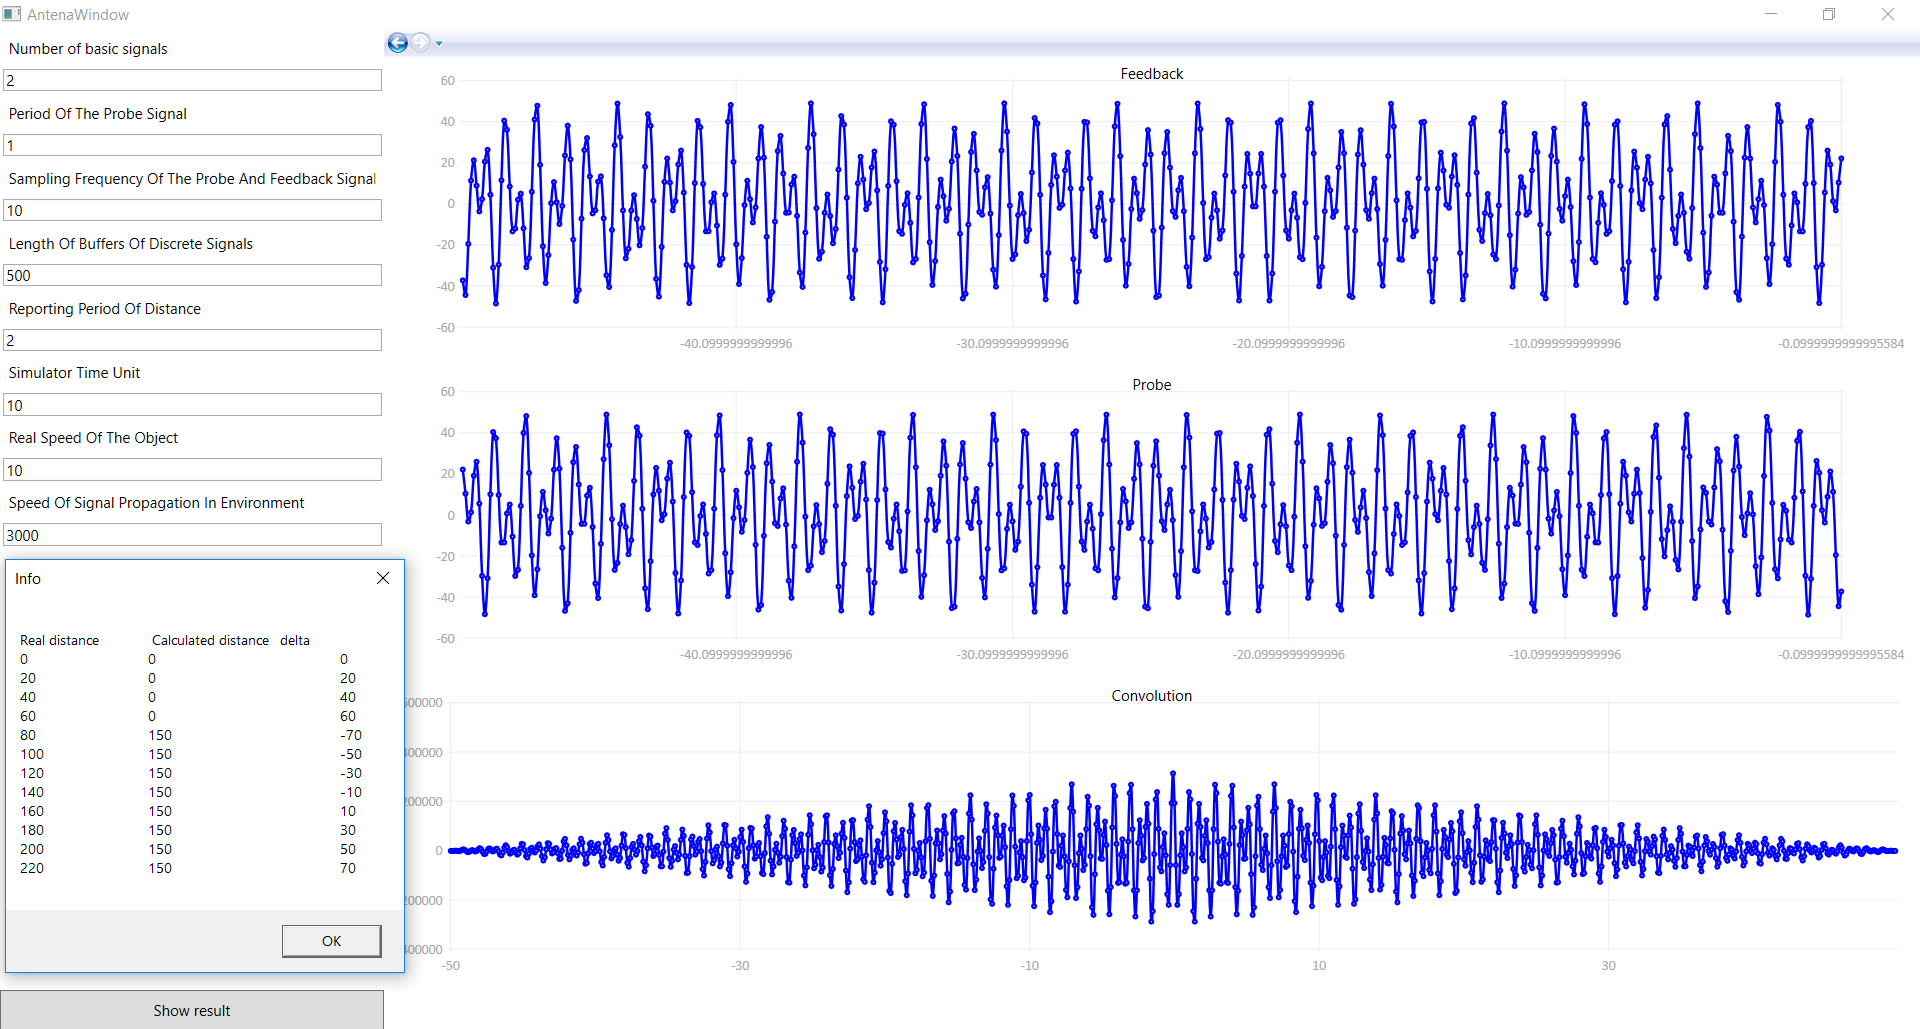
\includegraphics[width=14cm]{images/a2.PNG}
 \vspace{-0.3cm}
 \caption{Korelacyjny czujnik odległosci}
 \label{gui}
\end{figure}


\begin{figure}[H]
 \centering
 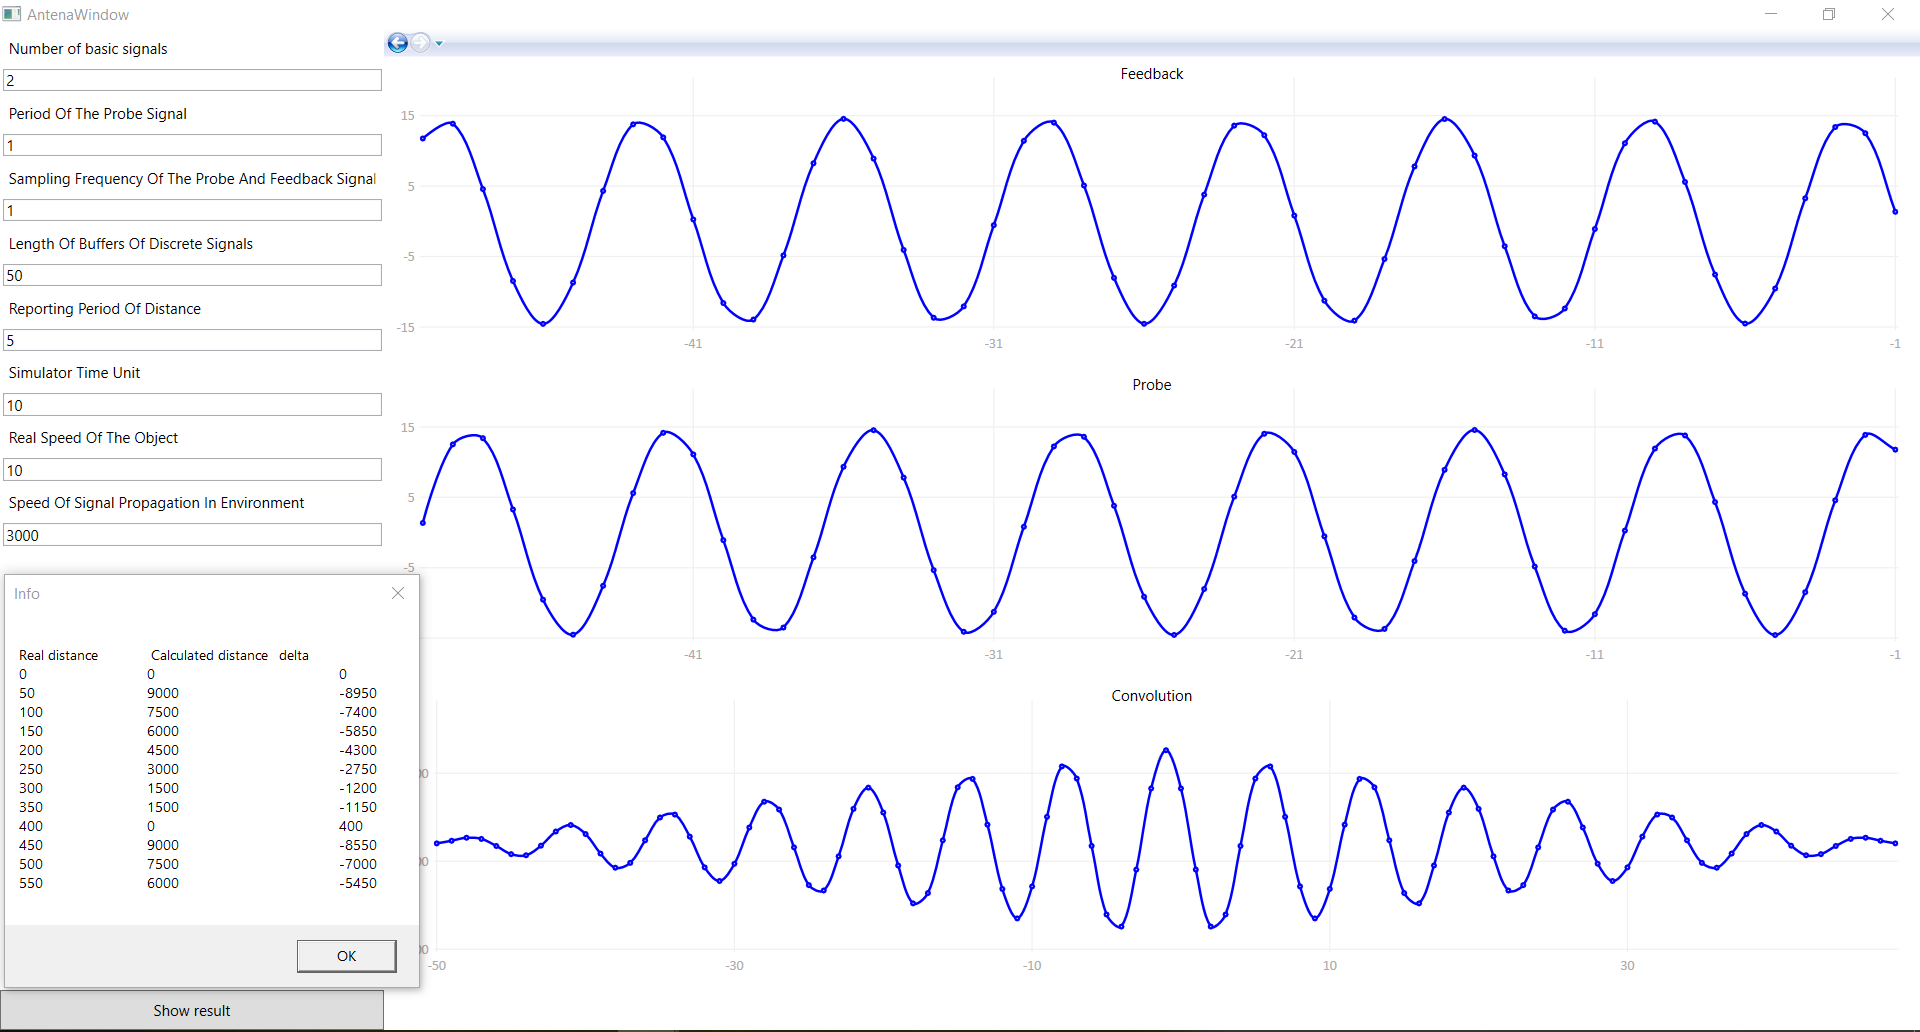
\includegraphics[width=14cm]{images/a3.PNG}
 \vspace{-0.3cm}
 \caption{Korelacyjny czujnik odległosci}
 \label{gui}
\end{figure}


\newpage

\section{Wnioski}

Aplikacja została napisania zgodnie z instrukcją zadania \cite{zad}. Aplikacja pozwala na rozszerzanie jej o kolejne funkcjonalnosci na potrzeby kolejnych zadań. 

Dla korelacyjnego czujnika odłegłosci kluczowe jest dobranie odpowiednio dużej częstotliwosci próbkowania, inaczej odległosć jest obliczana z dużym błędem.




%%%%%%%%%%%%%%%%%%%%%%%%%%%%%%%%%%%%%%%%%%%%%%%%%%%%%%%%%%%%%%%%%%%%%%%%%%%%%%%%%%%%%%%%%%%%%%%%%%%%%%%%%%%%%%%%%
% BIBLIOGRAFIA
%%%%%%%%%%%%%%%%%%%%%%%%%%%%%%%%%%%%%%%%%%%%%%%%%%%%%%%%%%%%%%%%%%%%%%%%%%%%%%%%%%%%%%%%%%%%%%%%%%%%%%%%%%%%%%%%%

\begin{thebibliography}{99}
\bibitem{pa} H.~Partl:
\emph{German \TeX},
TUGboat Vol.~9,, No.~1 ('88)
\bibitem{lv} Biblioteka LiveCharts. https://lvcharts.net
\bibitem{wpf} Windows Presentation Foundation. https://docs.microsoft.com/plpl/dotnet/framework/wpf/getting-started/walkthrough-my-frst-wpfdesktop-application
\bibitem{zad} https://ftims.edu.p.lodz.pl/pluginfile.php/13449/mod\_resource/content/0/zadanie3.pdf
\end{thebibliography}

\end{document}
